% The New Small Wheel (NSW) is a new detector system that was installed in the MS during the second long shutdown and is the first large upgrade to the ATLAS detector in preparation for the HL-LHC\@. The NSW is a set of precision tracking (Micromegas) and trigger detectors (sTGC) that are able to work at the high rates needed for the HL-LHC but also give excellent spatial and time resolution. This system consists of 16 detector planes that are arranged into two multilayers where each multilayer consists of four sTGC and four MM\@. To maximize the distance between the sTGCs for better track segment angular resolution at the trigger level, each multilayer is arranged in a sandwich configuration of sTGC-MM-MM-sTGC\@. The 16 detector sectors are subdivided into eight large sectors and 8 small sectors that alternate to ensure full cover in the $\varphi$ plane. The NSW can be seen in Figure~\ref{fig:atlas_nsw}.

% \begin{figure}[htp]
%     \centering
%     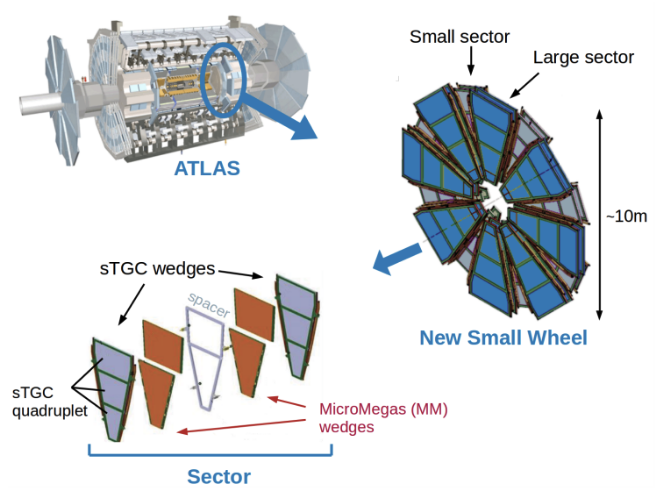
\includegraphics[width=0.65\textwidth]{figures/atlas/atlas_NSW.png}
%     \caption{Depicted is the NSW and its placement within the ATLAS detector. The figure illustrates the division of the NSW into 16 sectors, alternating between large and small sectors, as well as the internal structure of each sector. The sandwich-like arrangement of the detector planes, designed to maximize the separation between the sTGC wedges for improved angular resolution, is also visible. Taken from~\cite{NSW_image}.}\label{fig:atlas_nsw}
% \end{figure}

% The sTGC's are the primary trigger detectors in the NSW\@. They are based on the same principle as the TGC's that are used throughout the muon system except with smaller readout strips. The strips in the sTGC are 3.2 mm in pitch, significantly smaller than the TGC strips, providing improved angular resolution. In addition to strips the sTGC have another readout technology, copper pads. These pads have a significantly larger pitch of about 80 mm, and are used for the identification of muon tracks that roughly point to the IP\@.

% In contrast, the MM detectors serve as the primary precision trackers for the NSW\@. Each MM consists of a drift region defined by a copper cathode and a woven metallic mesh with an applied electric field of 600 V/cm applied between these. When an charged particle crosses this volume, an electron ion pair is created which drifts towards the mesh. An anode readout is placed below the mesh separated by a 129 $\mu$m amplification volume where there is an additional electric field of 40 kV/cm. The electric field configuration in the MM guides the electron to the amplification region, where an avalanche occurs, generating a charge signal on the readout.

%%%%%%%%%%%%%%%% revision

The New Small Wheel (NSW) was installed during LS2 and is the first major upgrade to ATLAS in preparation for the HL-LHC\@. It combines precision tracking chambers (Micromegas, MM) and trigger chambers (small-strip TGC,sTGC) that are able to meet the HL-LHC high rate and resolution demands. Each NSW consists of 16 sectors (8 large, 8 small) arranged alternatively in $\varphi$, with each sector containing two multilayers in a sTGC-MM-MM-sTGC sandwich for improved angular resolution. The NSW can be seen in Figure~\ref{fig:atlas_nsw}.

\begin{figure}[htp]
    \centering
    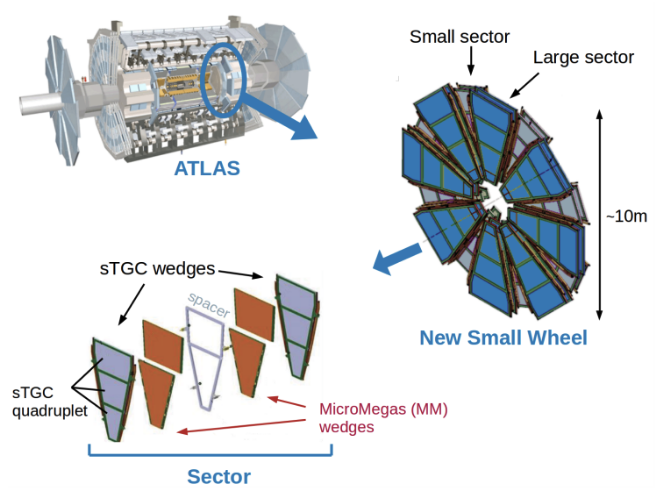
\includegraphics[width=0.65\textwidth]{figures/atlas/atlas_NSW.png}
    \caption{Depicted is the NSW and its placement within the ATLAS detector. The figure illustrates the division of the NSW into 16 sectors, alternating between large and small sectors, as well as the internal structure of each sector. The sandwich-like arrangement of the detector planes, designed to maximize the separation between the sTGC wedges for improved angular resolution, is also visible. Taken from~\cite{NSW_image}.}\label{fig:atlas_nsw}
\end{figure}

The sTGC's are the primary trigger detectors in the NSW\@. They are built upon the TGC technology but feature strips that are 3.2 mm in pitch and 80 mm copper pads for identifying muon tracks that roughly point to the IP. The MMs serve as the NSWs primary precision trackers and consist of a drift region defined by a copper cathode and a woven metallic mesh with an applied electric field of 600 V/cm. Below the mesh is an anode readout that is separated by a 129 $\mu$m amplification volume where an additional electric field of 40 kV/cm is applied. The amplification gap produces a localized avalanche signal that is read out by the anode.
